Até o momento, os desenhos experimentais discutidos assumem que a aleatorização é realizada no nível do indivíduo, onde cada unidade, como um aluno, é aleatorizada para receber ou não o tratamento. Por exemplo, no caso empírico analisado, os alunos são aleatorizados para determinar quem receberá uma vaga em uma escola de ensino técnico, permitindo uma análise causal direta no nível individual. No entanto, há situações em que, embora tenhamos dados a nível de indivíduo, a aleatorização é feita em um nível mais agregado. Imagine, por exemplo, que em vez de aleatorizar os alunos, a unidade de aleatorização passe a ser as escolas. Nesse caso, estaríamos aleatorizando escolas inteiras para receberem a implementação de um sistema de ensino técnico, enquanto ainda teríamos acesso aos dados individuais dos alunos que pertencem a essas escolas. 

Esse tipo de desenho exige ajustes específicos na especificação econométrica, pois a aleatorização em clusters (como escolas) cria dependências entre as observações dentro de cada unidade. Essas dependências se refletem nas correlações intraclasse (Intracluster Correlation - ICC) mede o quanto as observações dentro de um mesmo grupo (cluster) são parecidas entre si. Se os alunos de uma mesma escola tendem a ter notas mais parecidas entre si (por exemplo, devido ao mesmo professor, estrutura da escola ou ambiente socioeconômico), então existe uma alta ICC. Se as notas dos alunos dentro da mesma escola variam bastante, a ICC é baixa.

Para capturar corretamente essa estrutura, podemos especificar nossa regressão de forma a refletir essa hierarquia, considerando as correlações intraclasse e garantindo a robustez das inferências da seguinte maneira:

\begin{equation}
    Y_{ij} = \beta_0 + \beta_1 D_j + \nu_j + \eta_{ij}
\end{equation}

\noindent onde $i$ se refere ao aluno e $j$ se refere à escola. Por simplicidade, assuma que $\nu_j$ é \textit{i.i.d} e $\mathrm{Var}(\nu_j) = \tau^2$, e que $\eta_{ij}$ é \textit{i.i.d} e $\mathrm{Var}(\eta_{ij}) = \omega^2$. Ainda, assuma que temos $J$ escolas com $n$ alunos em cada. Novamente, estamos interessados em estimar $\beta_1$. Nesse caso, a variância do nosso estimador de MQO se torna

\begin{equation}\label{varcluster}
    \mathrm{Var}(\hat{\beta}_1) = \frac{1}{p(1-p)} \frac{n\tau^2 + \omega^2}{nJ}
\end{equation}

A partir da equação \ref{varcluster}, podemos derivar a fórmula do MDE para o caso de aleatorização a nível de grupo:

\begin{equation}\label{mde4}
    MDE = (t_{\frac{\alpha}{2}} + t_{1-\kappa})\sqrt{\frac{1}{p(1-p)} \frac{n\tau^2 + \omega^2}{nJ}}
\end{equation}

Podemos, também, derivar uma fórmula do MDE que se compare com o caso de um desenho de experimento em que a aleatorização tenha sido feita a nível de indivíduo. Com a notação introduzida nesta subseção, podemos escrever a variância do estimador de MQO para o caso de aleatorização a nível de indivíduo como

\begin{equation}\label{varclusterind}
    \mathrm{Var}(\hat{\beta}_{1, individuo}) = \frac{1}{p(1-p)} \frac{\tau^2 + \omega^2}{nJ}
\end{equation}

Ao dividirmos a equação \ref{varcluster} pela equação \ref{varclusterind}, obtemos o \textit{efeito do desenho} (Design Effect - DE), isto é, o efeito na variância do estimador de estarmos aleatorizando a nível de grupo comparado com aleatorizarmos a nível de indivíduo:

\begin{equation}\label{designeffect}
    DE = 1 + (n-1)\rho
\end{equation}

\noindent onde $\rho = \frac{\tau^2}{\tau^2 + \omega^2}$ é a correlação intraclasse (Intracluster Correlation - ICC). Podemos ver que, ao aleatorizarmos a nivel de grupo, a variância do nosso estimador de MQO estará aumentando tanto com $\rho$, quanto com $n$. Com isso, podemos derivar uma fórmula para o MDE em função do MDE com aleatorização a nível de indivíduo (Equação \ref{mde2}) e do efeito do desenho:

\begin{equation}\label{mde5}
    MDE = (t_{\frac{\alpha}{2}} + t_{1-\kappa})\sqrt{\frac{1}{p(1-p)}\frac{\sigma^2}{nJ}(1 + (n-1)\rho)}
\end{equation}

Se desconsiderarmos a correlação intraclasse em desenhos com aleatorização a nível de grupo, estaremos subestimando a variância do nosso estimador e, portanto, subestimando o MDE. Como observações dentro do mesmo cluster são mais parecidas, é como se tivéssemos menos ``dados úteis'' do que o número total de observações sugere.

Note que estes resultados de MDE dependem da hipótese de que $J$ e $n$ estão fixos. Porém, muitas vezes, por restrições da natureza do experimento, podemos ter tanto $J$, quanto $n$ variando por grupo de tratamento. Por exemplo, se tivermos o orçamento limitado, podemos aleatorizar menos escolas para receber o tratamento. Isso faria com que $J_1 < J_0$, o que irá mudar a variância do estimador de MQO e, por consequência, o MDE. Neste caso, a fórmula do MDE seria

\begin{equation}\label{mde6}
    MDE = (t_{\frac{\alpha}{2}} + t_{1-\kappa})\sqrt{\sigma^2(1 + (n-1)\rho)\left(\frac{1}{nJ_0}+\frac{1}{nJ_1}\right)}
\end{equation}

O mesmo pode ocorrer com nosso o número médio de indivíduos por cluster, $n$. Se esse número for diferente a depender do grupo de tratamento, o MDE é

\begin{equation}\label{mde7}
    MDE = (t_{\frac{\alpha}{2}} + t_{1-\kappa})\sqrt{\sigma^2\left(\frac{1-\rho}{n_1 J}+\frac{1+(2n_0 - 1)\rho}{n_0 J}\right)}
\end{equation}

\subsection{\sc Praticando: Fórmula Analítica}

Nesta seção, iremos calcular o MDE através da formula analítica para o caso de Clustered RCT. Como nas seções anteriores, iremos começar o código limpando o ambiente, carregando os pacotes necessários e definindo os parâmetros fixos no cálculo do MDE.


\begin{boxH}
\begin{lstlisting}[language = R]
# Limpar o ambiente 
rm(list=ls())

# Carregando pacotes necessários
library(tidyverse)

# Parâmetros para cálculo analítico do MDE
t.kappa = 0.84 # poder de 80%
t.alpha = 1.96 # nível de significância de 5%
P = 0.5 # Porcentagem de tratados de 50%
\end{lstlisting}
\end{boxH}

Agora, criaremos a função \texttt{MDE.cluster}, baseada na equação \eqref{mde5}. Iremos permitir que três argumentos variem nessa função: \texttt{N}, referente ao número médio de alunos dentro de uma escola, $N$; \texttt{J}, referente ao número de escolas na amostra, $J$; e \texttt{rho}, referente ao valor do ICC, $\rho$.

\begin{boxH}
\begin{lstlisting}[language = R]
# Fórmula do MDE variando N, J e ICC

MDE.cluster = function(N,J,rho){(t.kappa+t.alpha)*((1/(P*(1-P)))^0.5)*((1/(N*J))^0.5*(1+(N - 1)*rho)^0.5)}


\end{lstlisting}
\end{boxH}

Iremos produzir dois gráficos, um variando o número médio de alunos dentro das escolas, $N$, e outro variando o número de escolas na amostra, $J$. Ambos os gráficos contarão com três curvas para diferentes valores de ICC. O bloco de código abaixo faz o gráfico da Figura \ref{sfig:mdeN}, em que calculamos o MDE variando o número médio de alunos, $N$, de 10 a 70. Fixamos o número de escolas em 50, além de três valores diferentes de ICC: 0.05, 0.1 e 0.15.

\begin{boxH}
\begin{lstlisting}[language = R]
# Gráfico do MDE variando N, para ICC de 0.05, 0.1 e 0.15, com J = 50

ggplot() + xlim(10, 70) +
  geom_function(fun = MDE.cluster, args = list(J = 50, rho = 0.05), aes(colour = "ICC = 0.05"), linewidth = 0.8) +
  geom_function(fun = MDE.cluster, args = list(J = 50, rho = 0.1), aes(colour = "ICC = 0.1"), linewidth = 0.8) +
  geom_function(fun = MDE.cluster, args = list(J = 50, rho = 0.15), aes(colour = "ICC = 0.15"), linewidth = 0.8) +
  labs(y = "MDE", x = "N") +
  theme_classic() +
  guides(colour=guide_legend(title="ICC"))


\end{lstlisting}
\end{boxH}

O segundo gráfico, produzido pelo bloco de código abaixo, está representado na Figura \ref{sfig:mdeJ}. Nela calculamos o MDE variando o número de escolas da amostra, $J$, de 10 a 70, mantendo o número médio de alunos nas escolas fixo em 30 e para os mesmos três valores de ICC. Note que, em ambos os casos, quanto maior o ICC, maior o MDE. 

\begin{boxH}
\begin{lstlisting}[language = R]
# Gráfico do MDE variando J, para ICC de 0.05, 0.1 e 0.15, com N = 30

ggplot() + xlim(10, 70) +
  geom_function(fun = MDE.cluster, args = list(N = 30, rho = 0.05), aes(colour = "ICC = 0.05"), linewidth = 0.8) +
  geom_function(fun = MDE.cluster, args = list(N = 30, rho = 0.1), aes(colour = "ICC = 0.1"), linewidth = 0.8) +
  geom_function(fun = MDE.cluster, args = list(N = 30, rho = 0.15), aes(colour = "ICC = 0.15"), linewidth = 0.8) +
  labs(y = "MDE", x = "J") +
  theme_classic() +
  guides(colour=guide_legend(title="ICC"))

\end{lstlisting}
\end{boxH}

\begin{figure}[h]
    \centering
    \begin{subfigure}{0.49\textwidth}
        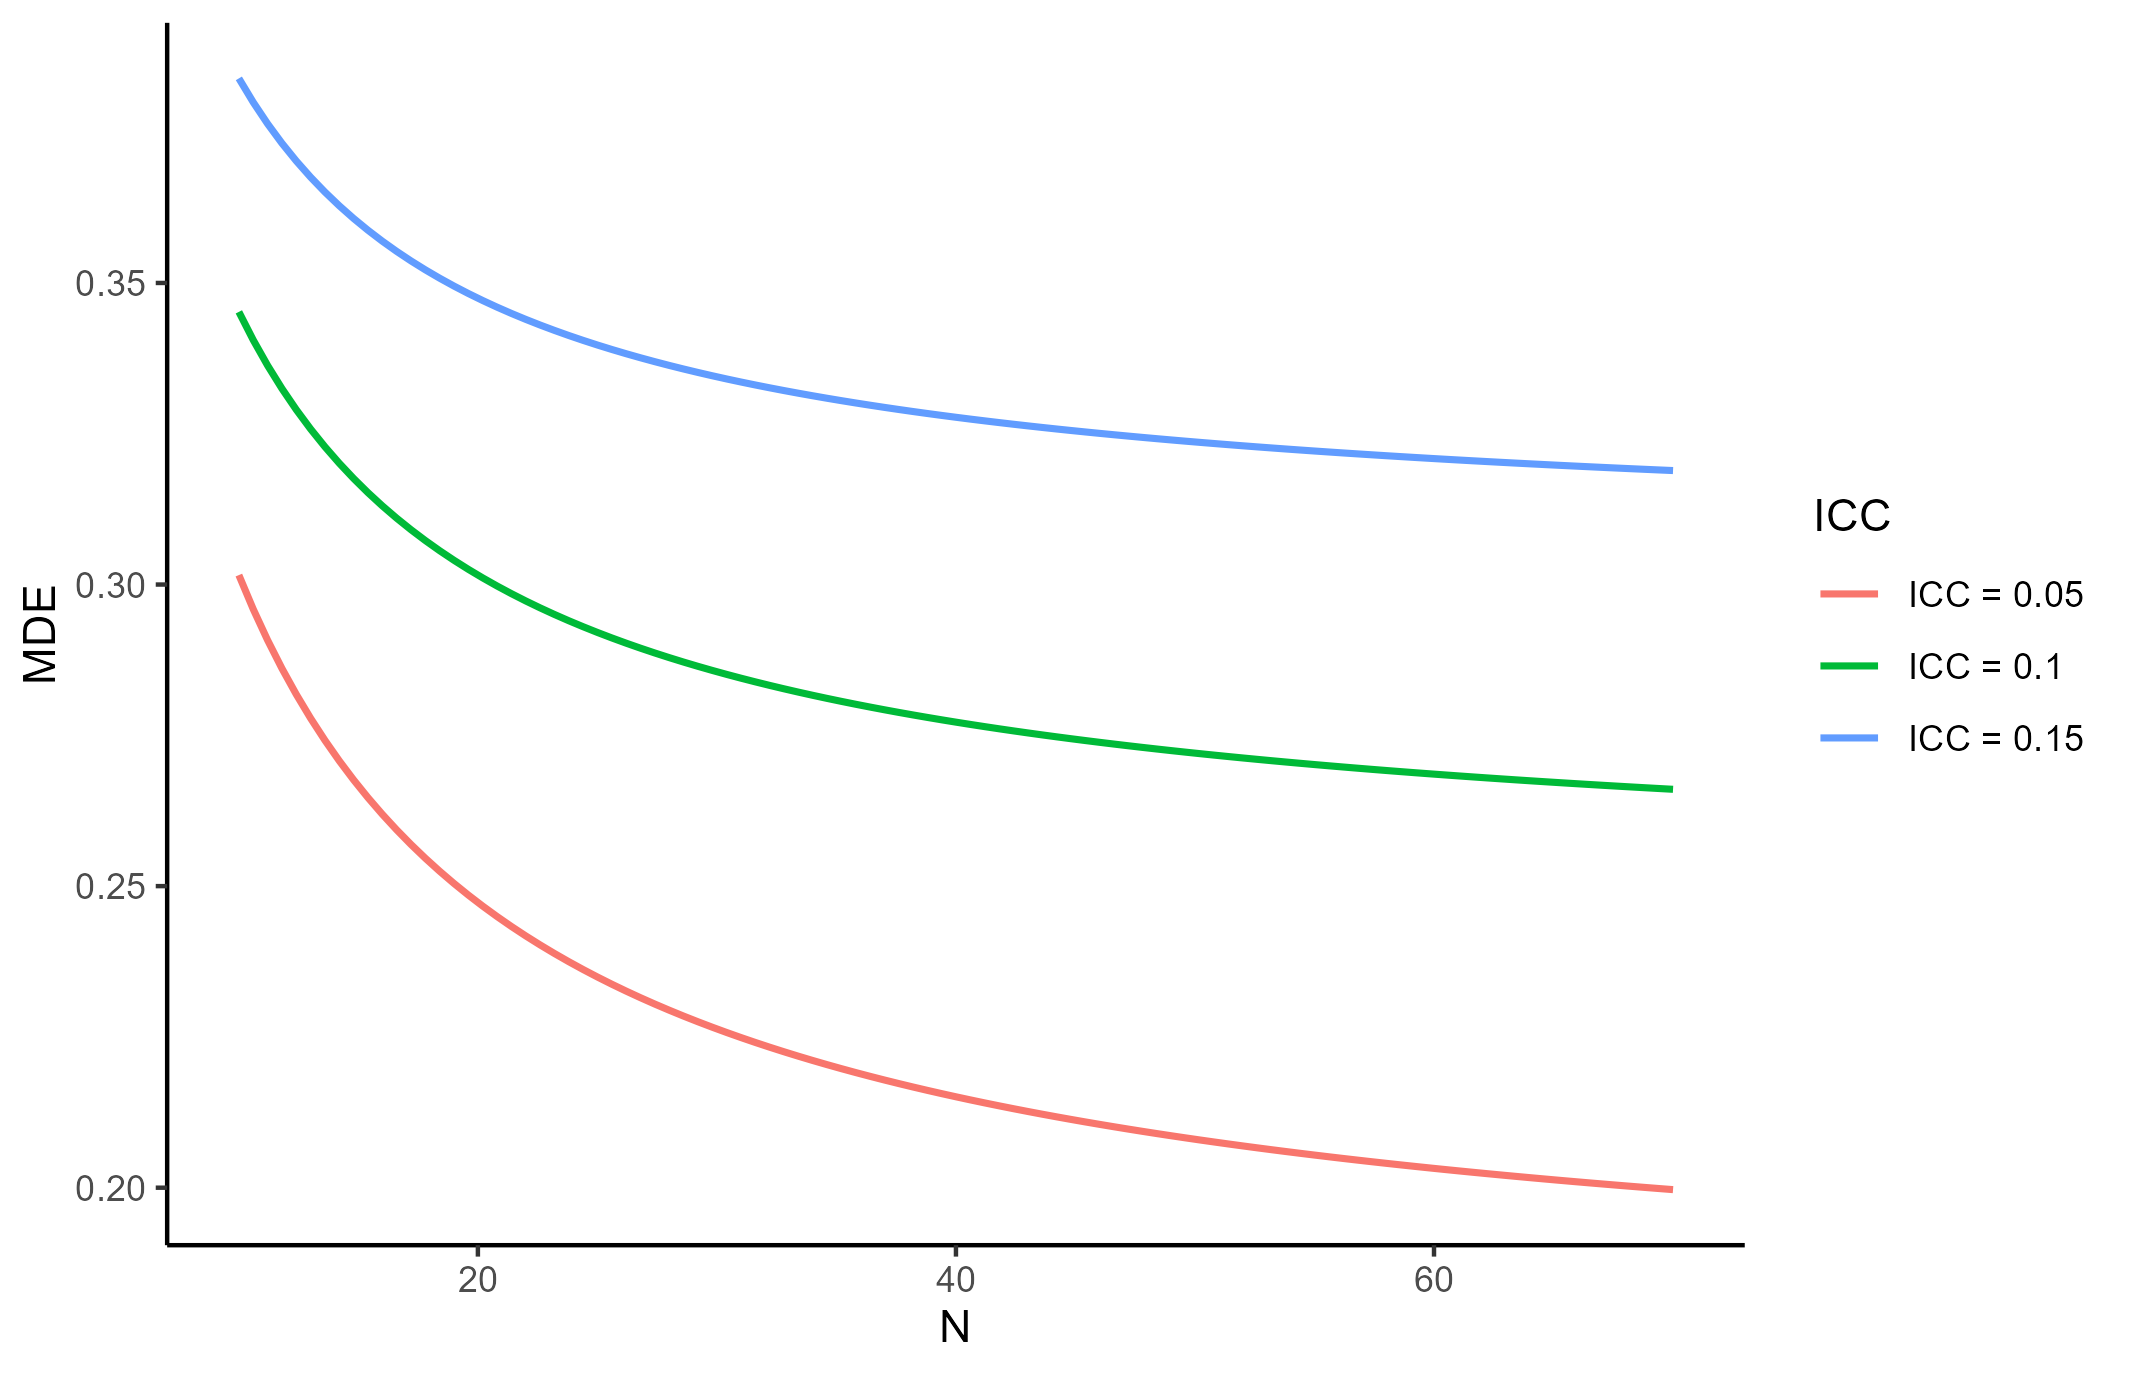
\includegraphics[width=\linewidth]{Figuras/mde_N_cluster.png}
        \caption{Gráfico de MDE variando $N$ para diferentes valores de ICC.}
        \label{sfig:mdeN}
    \end{subfigure}
   \begin{subfigure}{0.49\textwidth}
        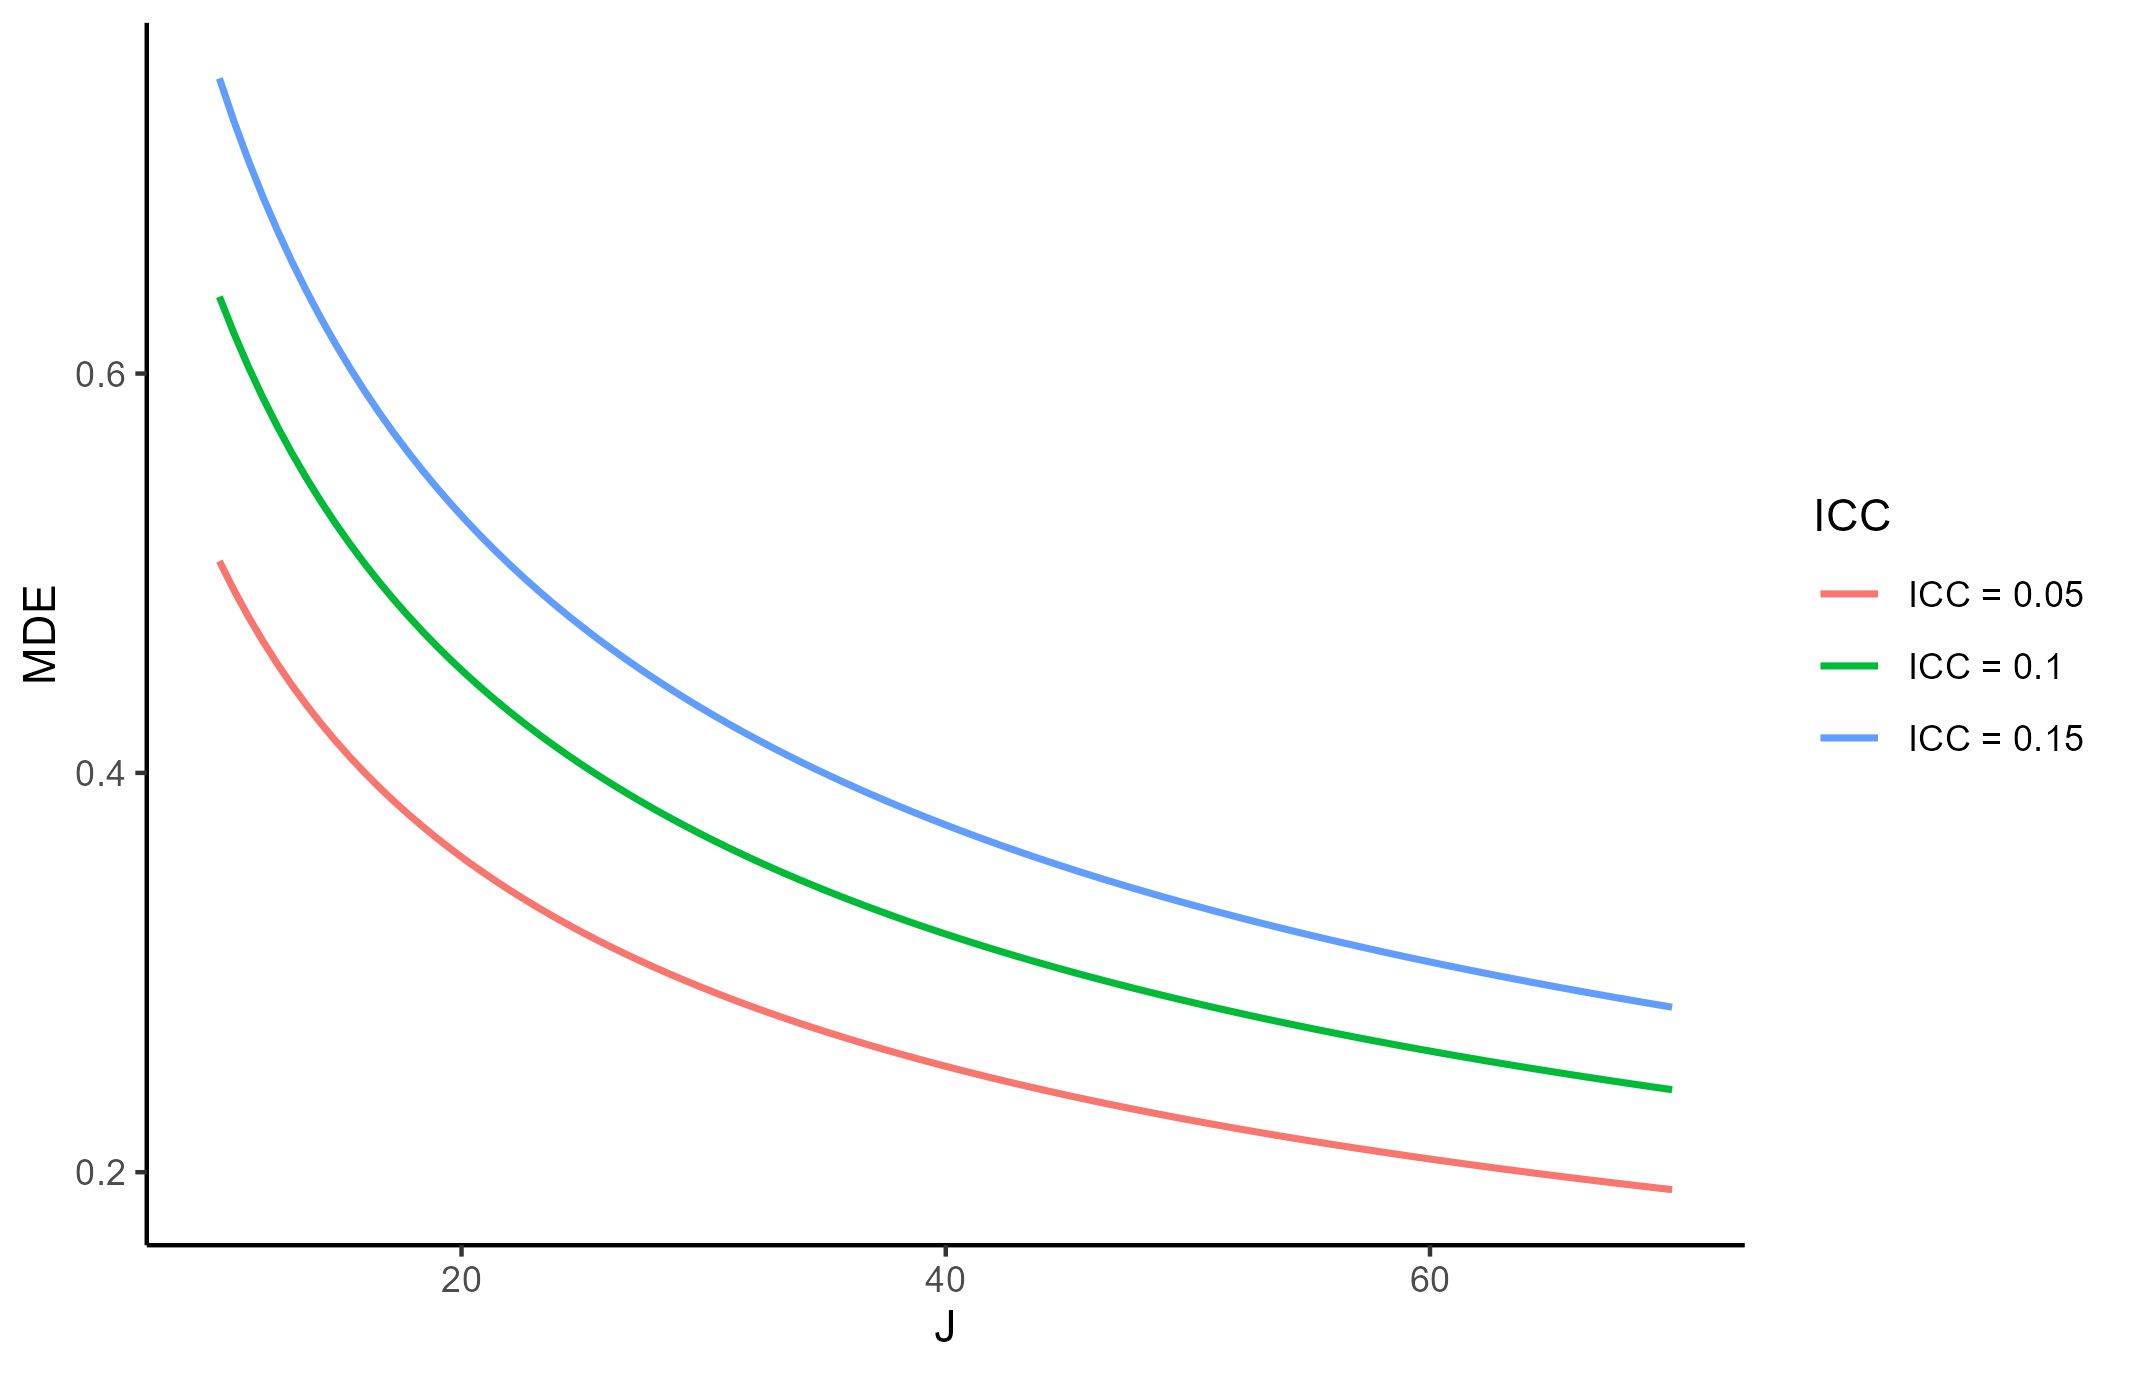
\includegraphics[width=\linewidth]{Figuras/mde_J_cluster.png}
        \caption{Gráfico de MDE variando $J$ para diferentes valores de ICC.}
        \label{sfig:mdeJ}
    \end{subfigure}
    \caption{Gráficos de MDE variando o número médio de alunos e o número de escolas da amostra para diferentes valores de ICC.}
    \label{fig:enter-label}
\end{figure}

\subsection{\sc Praticando: Simulações}

Nesta seção, iremos calcular o MDE de forma simulada para o caso de Clustered RCT. Como das outras vezes, iremos limpar o ambiente de trabalho, carregar os pacotes necessários, escolher uma \textit{seed} aleatória e carregar a base de dados. Desta vez, utilizaremos também o pacote \texttt{lfe} para as estimativas dos erros padrões levarem o nível do cluster em consideração. Ainda, importaremos a base \texttt{base\_rct\_cluster.csv}.

\begin{boxH}
\begin{lstlisting}[language = R]
# Limpar o ambiente 
rm(list=ls())

# Carregando pacotes necessários

library(tidyverse)
library(randomizr)
library(lfe)

# Fazendo com que as simulações se tornem reproduzíveis
set.seed(42)

# Base de dados
base_rct_cluster <- read.csv("Base/base_rct_cluster.csv")
\end{lstlisting}
\end{boxH}

O bloco de código abaixo estima o erro padrão do estimador de efeito fixo por meio de simulações. A grande diferença em relação às seções anteriores é o fato de que iremos aleatorizar o tratamento a nível de escola. Com as escolas aleatorizadas, iremos rodar uma regressão clusterizando o erro padrão a nível de escola, armazenaremos os erros padrões e calcularemos o MDE a partir da média desses erros padrões estimados.

\begin{boxH}
\begin{lstlisting}[language = R]
# Criando vetor com 100 entradas para armazenar os erros padrões
se_cluster <- c(rep(NA, 100))

# Simulando 100 vezes o erro padrão
for (i in 1:100) {
  
  # aleatorizando escolas
  D <- simple_ra(N = length(unique(base_rct_cluster$id_escola)), prob = 0.5) 
  
  # criando base para dar match na base principal
  match <- data.frame(id_escola = unique(base_rct_cluster$id_escola),
                      D = D)
  df <- left_join(base_rct_cluster, match, by = "id_escola") #juntando bases
  
  reg_cluster <- felm(y ~ D|0|0|id_escola, data = df) # regressão
  se_cluster[i] <- summary(reg_cluster)$coefficients[2,2] #armazenando se
  
}

# Calculando MDE
MDE_cluster = 2.8*mean(se_cluster)
print(MDE_cluster)
\end{lstlisting}
\end{boxH}